\section{Discussion}

\paragraph{Key insight.}
Our central finding is that \textit{designed information asymmetry} is necessary for effective multi-agent deliberation.
When all agents receive identical evidence, iterative discussion provides little measurable benefit, as agents merely reinforce correlated beliefs rather than contribute complementary knowledge (Figure~\ref{fig:herding}).
This aligns with the martingale characterization of homogeneous-input debate and suggests that the widely adopted practice of giving all agents the same context fundamentally limits the value of multi-agent interaction.

\paragraph{Future work.}
Natural extensions include (1)~adaptive routing that dynamically adjusts evidence allocation based on emerging disagreement, (2)~more expressive routing algorithms beyond BM25, such as dense retrieval or learned semantic partitioning, (3)~learned aggregation replacing the fixed shrinkage parameters, (4)~evaluation on open-ended and multi-choice forecasting tasks, and (5)~heterogeneous model panels that leverage model-level diversity in addition to evidence-level asymmetry.

\paragraph{Potential risks.}
Designed information asymmetry encourages agents to maintain distinct beliefs, but it may also amplify biased or misleading evidence partitions. If private evidence subsets contain low-quality, adversarial, or outdated documents, agents may become confidently polarized around incorrect conclusions rather than self-correcting through deliberation. In addition, rationale sharing introduces a potential attack surface, where persuasive but flawed rationales propagate errors across agents. Future deployments should incorporate evidence verification, source reliability estimation, and safeguards against adversarial persuasion.

\section{\textsc{PolyGym} Benchmark Details}
\label{sec:appendix_dataset}

\paragraph{Motivation.}
Agentic forecasting systems for prediction markets require two distinct capabilities:
(1)~\textit{retrieval}, identifying relevant information from the web, and
(2)~\textit{utilization}, reasoning over that information to produce calibrated probability estimates.
Existing benchmarks predominantly evaluate these capabilities jointly (Table~\ref{tab:benchmark_comparison}), making it difficult to determine whether performance gains arise from better retrieval or better collective reasoning.
Live benchmarks~\citep{karger2024forecastbench,zeng2025futurex} additionally introduce variability from changing web environments and unstable evidence availability, and retrieval-augmented systems continue to exhibit degradation over time, suggesting that access to information alone does not solve the utilization challenge~\citep{dailyoracle}.
\textsc{PolyGym} therefore fixes the evidence pool: all methods observe the same pre-retrieved corpus, while different agents may observe different subsets of it.
Conceptually, this parallels controlled retrieval settings in QA research~\citep{chen2021finqa,yang2018hotpotqa} that separate retrieval quality from downstream reasoning.

\begin{figure}[H]
    \centering
    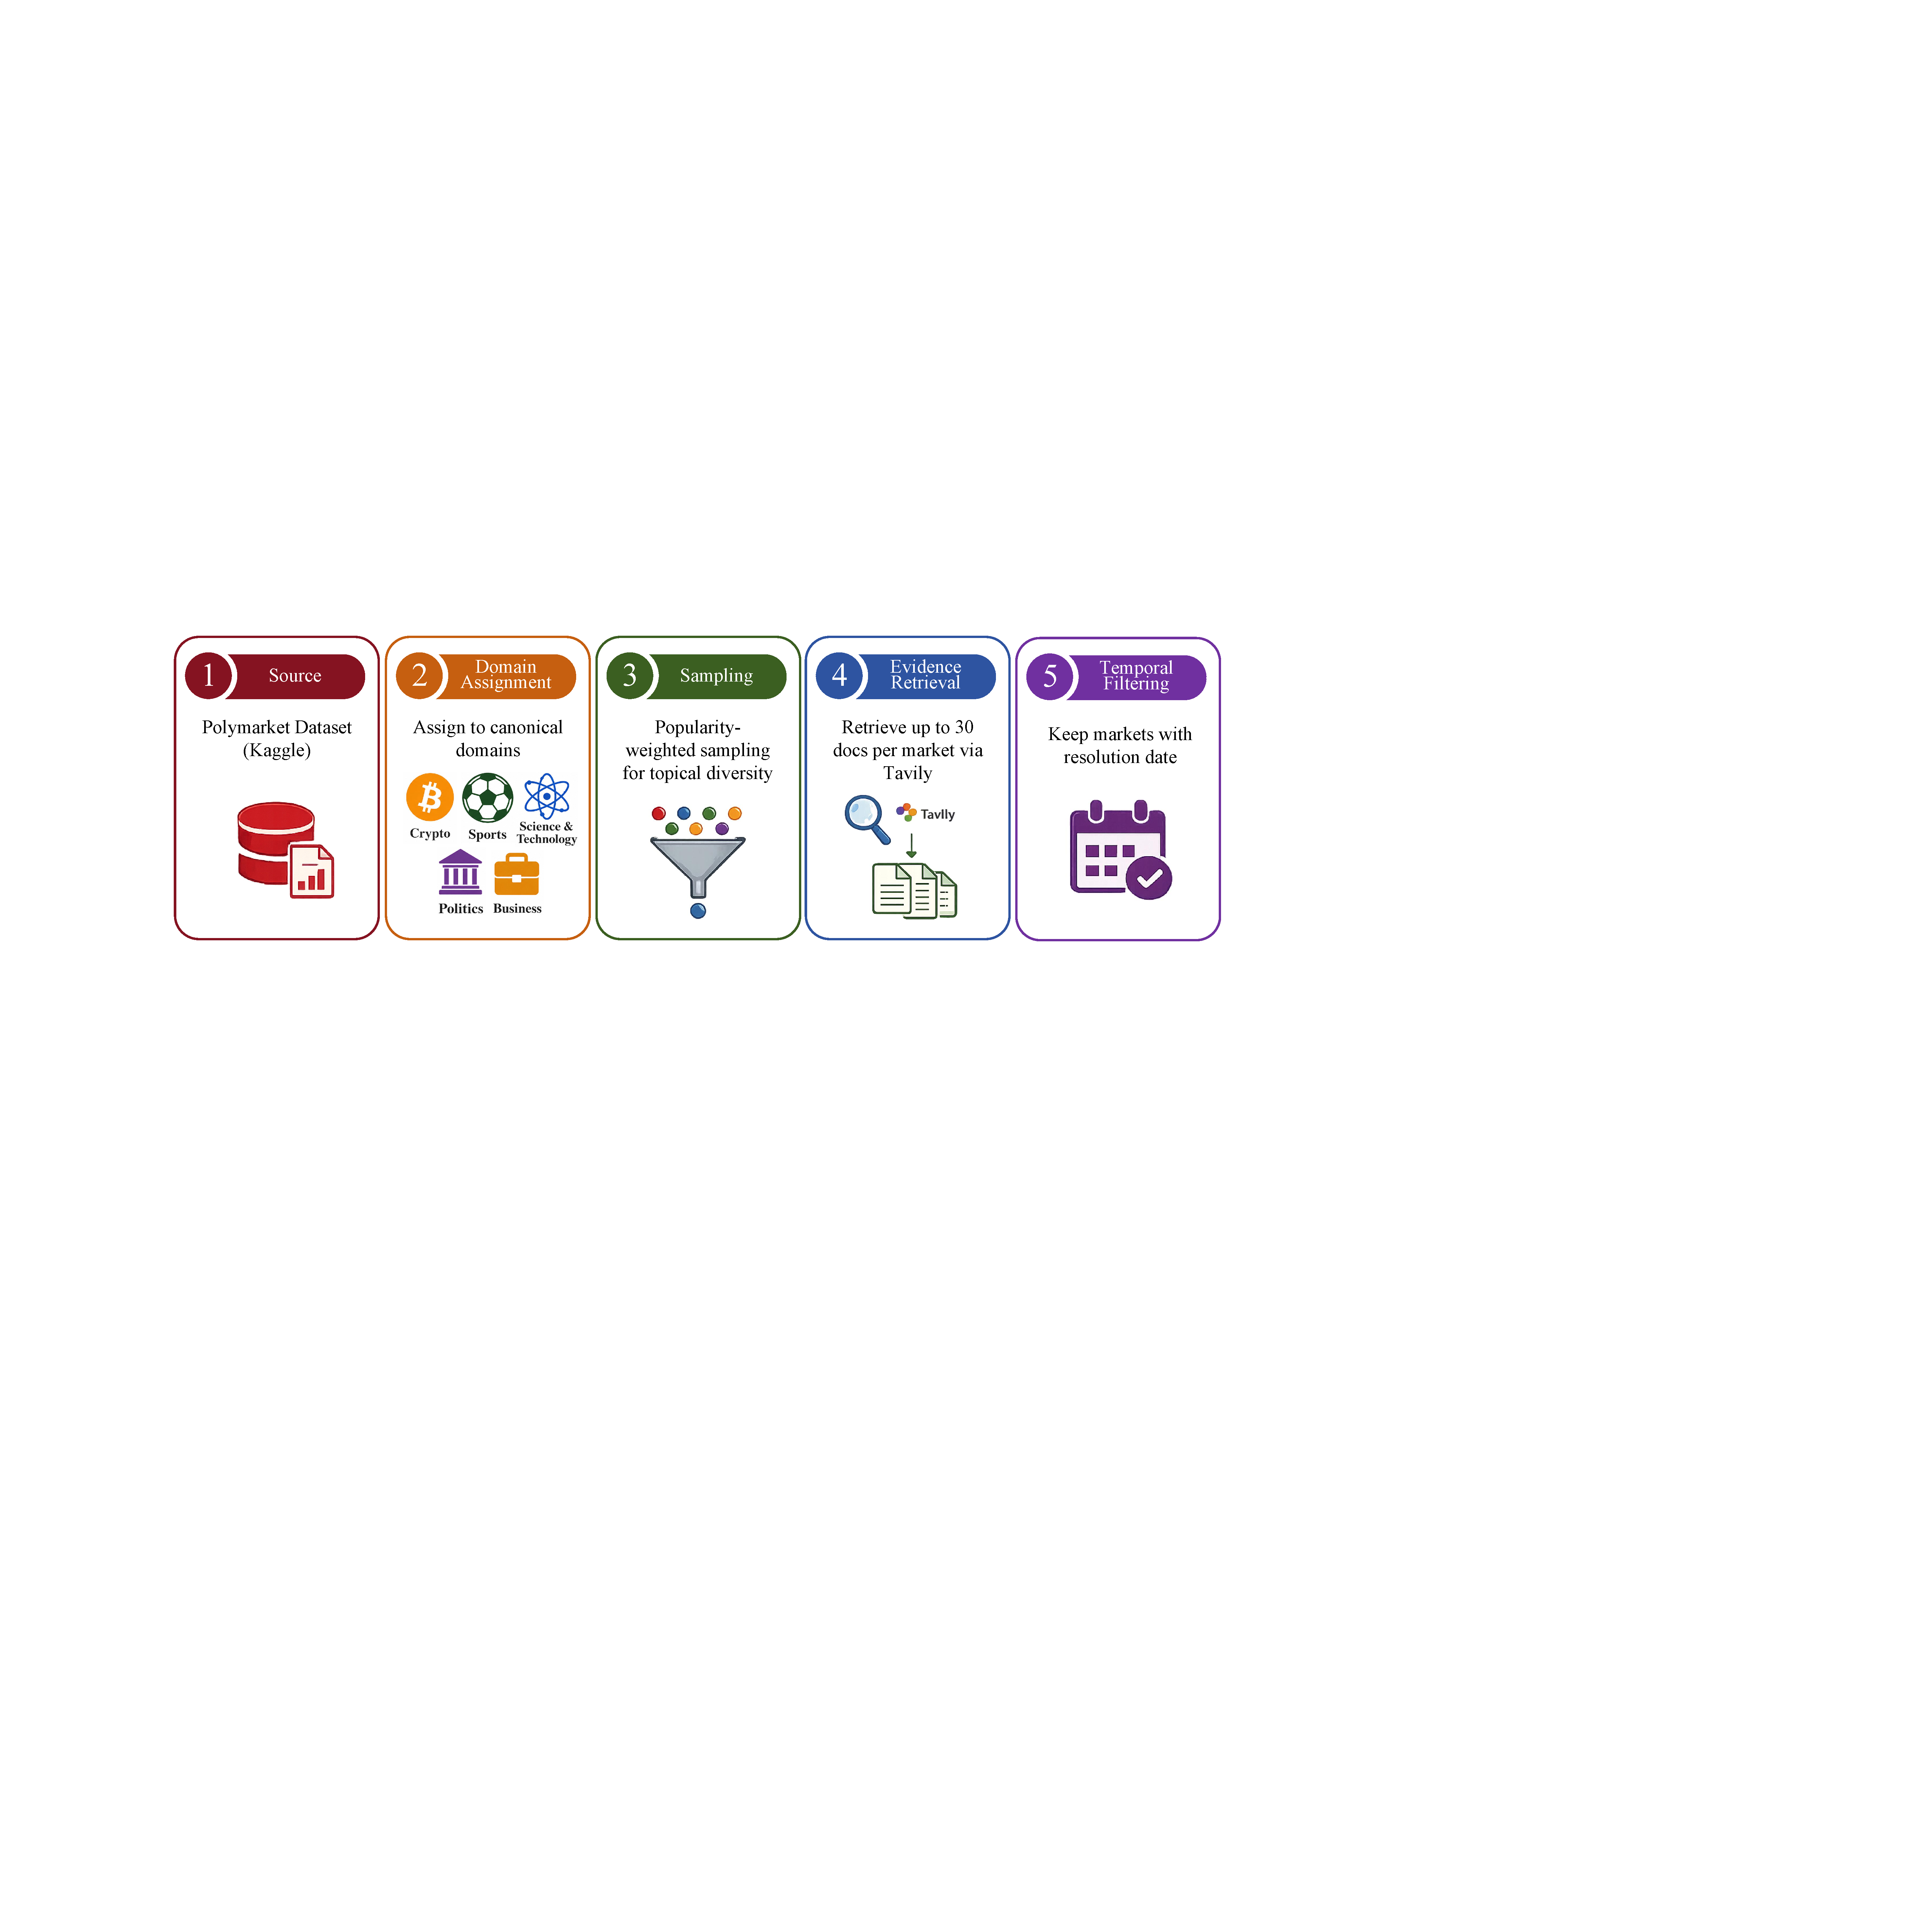
\includegraphics[width=1\linewidth]{figures/dataset.pdf}
    \caption{\textsc{PolyGym} data construction pipeline.}
    \label{fig:dataset}
\end{figure}

\begin{table*}[!ht]
\centering
\small
\resizebox{\textwidth}{!}{
\begin{tabular}{lcccccc}
\toprule
\textbf{Setup} & \textbf{Static} & \textbf{Reproducible} & \textbf{Time Control} & \textbf{Fixed Evidence} & \textbf{Realistic} & \textbf{Agent Study} \\
\midrule
ForecastBench~\citep{karger2024forecastbench} & \xmark & \xmark & \cmark & \xmark & \cmark & \xmark \\
FutureX~\citep{zeng2025futurex} & \xmark & \xmark & \cmark & \xmark & \cmark & \xmark \\
PolyBench~\citep{cheng2026polybenchbenchmarkingllmforecasting} & \xmark & \xmark & \cmark & \xmark & \cmark & \xmark \\
Prediction Arena~\citep{zhang2026predictionarenabenchmarkingai} & \xmark & \xmark & \cmark & \xmark & \cmark & \cmark \\
Zou et al.~\citep{zou2022forecasting} & \cmark & \xmark & \xmark & \xmark & \xmark & \xmark \\
Halawi et al.~\citep{halawi2024approaching} & \cmark & \xmark & \xmark & \xmark & \xmark & \xmark \\
\midrule
\textbf{\textsc{PolyGym} (Ours)} & \cmark & \cmark & \cmark & \cmark & \cmark & \cmark \\
\bottomrule
\end{tabular}
}
\caption{Comparison of forecasting evaluation setups. \textsc{PolyGym} provides fixed evidence and full reproducibility, enabling controlled study of information utilization and multi-agent deliberation.}
\label{tab:benchmark_comparison}
\end{table*}

\paragraph{Construction.}
\textsc{PolyGym} is derived from a large-scale Polymarket dataset~\citep{kaggle_polymarket_dataset} consisting of approximately 40{,}000 events and 100{,}000 prediction markets.
Events are assigned to canonical domains using metadata fields, and popularity-weighted sampling ensures topical diversity.
After temporal filtering (below), the benchmark contains 250 resolved binary markets: Sports (106), Business (28), Politics (23), Entertainment (6), Geopolitics (5), and other domains (82).
The empirical YES rate is 0.232.
All questions and evidence documents are in English.

\paragraph{Evidence.}
For each market, we retrieve up to 20 documents via the Tavily search API\footnote{\url{https://www.tavily.com/}} using queries derived from the question text (mean 19.5 documents per question).
A strict temporal cutoff ensures all evidence precedes the market resolution date.
Retrieved documents are deduplicated and truncated to 500 characters.

\paragraph{Temporal filtering.}
To reduce contamination from LLM prior knowledge, we retain only markets with resolution dates between 2025-09-09 and 2025-12-02, after the primary model's knowledge cutoff.

\paragraph{Licenses and intended use.}
The source Polymarket dataset~\citep{kaggle_polymarket_dataset} is licensed under the Open Data Commons Database Contents License (DbCL) v1.0.
Evidence documents retrieved via the Tavily Search API are used solely for non-commercial research purposes under its API terms of service and are not independently redistributed.
\textsc{PolyGym} is intended for research use only. The accompanying code is released under the MIT License.

\section{Proof of Proposition~\ref{prop:decorrelation}}
\label{sec:appendix_proof}

We provide the complete derivation.
Let $\epsilon_j = \rho \cdot \epsilon^{\mathrm{pub}} + (1 - \rho) \cdot \epsilon_j^{\mathrm{priv}}$ for agent $j \in \{1, \dots, J\}$.

\paragraph{Covariance between agents.}
For $i \neq j$, expanding by bilinearity of covariance:
\begin{align}
\mathrm{Cov}(\epsilon_i, \epsilon_j)
  &= \rho^2 \mathrm{Var}(\epsilon^{\mathrm{pub}}) \nonumber\\
  &\quad + \rho(1{-}\rho)\mathrm{Cov}(\epsilon^{\mathrm{pub}}, \epsilon_j^{\mathrm{priv}}) \nonumber\\
  &\quad + \rho(1{-}\rho)\mathrm{Cov}(\epsilon_i^{\mathrm{priv}}, \epsilon^{\mathrm{pub}}) \nonumber\\
  &\quad + (1{-}\rho)^2\mathrm{Cov}(\epsilon_i^{\mathrm{priv}}, \epsilon_j^{\mathrm{priv}}).
\end{align}
By the independence assumptions, $\mathrm{Cov}(\epsilon_i^{\mathrm{priv}}, \epsilon_j^{\mathrm{priv}}) = 0$
and $\mathrm{Cov}(\epsilon^{\mathrm{pub}}, \epsilon_j^{\mathrm{priv}}) = 0$, so
$\mathrm{Cov}(\epsilon_i, \epsilon_j) = \rho^2 \mathrm{Var}(\epsilon^{\mathrm{pub}})$.

\paragraph{Individual variance.}
Since $\epsilon^{\mathrm{pub}}$ and $\epsilon_j^{\mathrm{priv}}$ are independent, the cross term vanishes:
$\mathrm{Var}(\epsilon_j) = \rho^2 \mathrm{Var}(\epsilon^{\mathrm{pub}}) + (1{-}\rho)^2 \mathrm{Var}(\epsilon_j^{\mathrm{priv}})$.

\paragraph{Correlation.}
Let $\sigma_{\mathrm{pub}}^2 = \mathrm{Var}(\epsilon^{\mathrm{pub}})$ and assume agents are symmetric ($\mathrm{Var}(\epsilon_j^{\mathrm{priv}}) = \sigma_{\mathrm{priv}}^2$ for all $j$), which implies $\mathrm{Var}(\epsilon_i) = \mathrm{Var}(\epsilon_j)$ and simplifies the correlation to
\begin{equation}
\mathrm{Corr}(\epsilon_i, \epsilon_j)
  = \frac{\rho^2 \sigma_{\mathrm{pub}}^2}{\rho^2 \sigma_{\mathrm{pub}}^2 + (1{-}\rho)^2 \sigma_{\mathrm{priv}}^2}.
\end{equation}
In the homogeneous baseline where $\rho = 1$: $\mathrm{Corr}(\epsilon_i, \epsilon_j) = 1$.
As $\rho$ decreases, correlation decreases monotonically, reaching 0 when $\rho = 0$.
At our default $\rho = 0.5$ with equal-variance components, $\mathrm{Corr} = 0.5$, a 50\% reduction relative to $\rho = 1$. \qed

\section{Proof of Corollary~\ref{cor:tradeoff}}
\label{sec:appendix_corollary}

Define the \textit{communicability} between two agents as the mutual information between their forecast errors, $C(\rho) := I(\epsilon_i;\, \epsilon_j)$.
When $\rho = 0$, the private components are independent by assumption, so $C(0) = 0$.
For $\rho > 0$, agents share the common component $\epsilon^{\mathrm{pub}}$, so $C(\rho) > 0$.
By the Data Processing Inequality~\citep{shin2026reasoning}, $C(\rho)$ upper-bounds the information any function of $\epsilon_i$ (including agent $i$'s rationale) can provide to agent $j$: at $\rho = 0$, deliberation cannot transfer information between agents.

\paragraph{Ensemble MSE decomposition.}
Our objective is to find $\rho^* = \arg\min_{\rho \in [0,1]} L(\rho)$.
The $J$-agent ensemble MSE decomposes as
\begin{equation}
L(\rho) \;=\; \underbrace{\frac{\sigma^2(\rho)}{J}\bigl[1+(J{-}1)\,r(\rho)\bigr]}_{\text{variance term } V(\rho)}
\;+\; \underbrace{D(\rho)^2}_{\text{bias term}},
\end{equation}
where $\sigma^2(\rho) = \rho^2\sigma_{\mathrm{pub}}^2 + (1{-}\rho)^2\sigma_{\mathrm{priv}}^2$ is the individual agent variance and $r(\rho)$ is the inter-agent correlation from Proposition~\ref{prop:decorrelation}.
We model $D(\rho)$ as a continuous, non-increasing function of $C(\rho)$, with $D(0) = D_0$ (single-agent bias, since deliberation cannot transfer information when $C(0) = 0$) and $D(\rho) < D_0$ for all $\rho > 0$.

\paragraph{Boundary analysis.}
\textit{At $\rho = 1$}: $r(1) = 1$, so $V(1) = \sigma_{\mathrm{pub}}^2$, equal to single-agent variance with no ensemble gain.
For any $\rho = 1 - \varepsilon$ with $\varepsilon > 0$: $r(1{-}\varepsilon) < 1$, so $V(1{-}\varepsilon) < V(1)$, while $D(1{-}\varepsilon) \approx D(1)$ by continuity.
Therefore $L(1{-}\varepsilon) < L(1)$, and $\rho = 1$ is not a minimizer.

\textit{At $\rho = 0$}: $\sigma^2(0) = \sigma_{\mathrm{priv}}^2$, $r(0) = 0$, and $C(0) = 0$.
Differentiating,
$\left.\frac{d\sigma^2}{d\rho}\right|_{\rho=0} = -2\sigma_{\mathrm{priv}}^2 < 0$ and
$\left.\frac{dr}{d\rho}\right|_{\rho=0} = 0$
(the numerator of $r$ vanishes to second order at $\rho = 0$), so
\begin{equation}
\left.\frac{dV}{d\rho}\right|_{\rho=0} = -\,\frac{2\sigma_{\mathrm{priv}}^2}{J} \;<\; 0.
\end{equation}
By continuity there exists $\varepsilon_V > 0$ such that $V(\varepsilon) < V(0)$ for $\varepsilon \in (0, \varepsilon_V)$; simultaneously, $C(\varepsilon) > 0$ implies $D(\varepsilon) < D_0$.
Combining, $L(\varepsilon) < L(0)$ for sufficiently small $\varepsilon > 0$, so $\rho = 0$ is not a minimizer.

\paragraph{Existence of interior optimum.}
Since neither boundary is a minimizer and $L(\rho)$ is continuous on the compact interval $[0,1]$, the minimum is attained at some $\rho^* \in (0,1)$. \qed

\section{Experimental Details}
\label{sec:appendix_details}

\subsection{Baseline Descriptions}

\paragraph{\ding{224} Single-Agent Methods.}
\begin{itemize}[nosep]
    \item \textbf{Chain-of-Thought}~\citep{wei2022chain}: one agent receives all evidence and produces a forecast with chain-of-thought reasoning.
    \item \textbf{Self-Consistency}~\citep{wangself}: the same CoT prompt is sampled 5 times at temperature 0.7 and predictions are averaged.
    \item \textbf{Sequential Bayesian}~\citep{shi2023language}: evidence items are processed one at a time by $K{=}5$ sequential agents, each updating the previous agent's probability estimate.
    \item \textbf{Superforecaster}~\citep{karger2024forecastbench}: a structured reasoning prompt that instructs the model to decompose the question, estimate base rates, update with evidence, and perform a calibration check.
    \item \textbf{Halawi et al.}~\citep{halawi2024approaching}: a 7-step structured scratchpad prompt (rephrase, pro/con arguments, aggregate, calibration check) run 3 times, combined via a trimmed mean that downweights the prediction furthest from the median by 50\%.
\end{itemize}

\paragraph{\ding{224} Multi-Agent Methods (Homogeneous Input).}
\begin{itemize}[nosep]
    \item \textbf{Standard Debate}~\citep{du2023improving}: 3 agents all receive the full evidence corpus, deliberate over 2 rounds sharing predictions and rationales, with final predictions aggregated by mean. As noted in Section~\ref{sec:setup}, our implementation shares InfoDelphi's prompt and protocol and differs only in information structure.
    \item \textbf{MoA}~\citep{wangmixture}: 3 proposer agents independently forecast with full evidence; a 4th aggregator agent receives all proposals with rationales and produces a final synthesized prediction.
    \item \textbf{Crowd Ensemble}~\citep{schoenegger2024wisdom}: 5 independent agents each receive all evidence and predict; the median prediction is the final forecast.
    \item \textbf{AIA Forecaster}~\citep{alur2025aia}: 10 independent agents forecast with full evidence, and a supervisor agent identifies disagreements and produces a final prediction with a confidence label; on low confidence the system falls back to the mean of the 10 agents.
\end{itemize}

\subsection{Computational Cost}
A full InfoDelphi run on \textsc{PolyGym}-250 issues $250 \times 3 \times 2 = 1{,}500$ forecasting calls plus lightweight aggregation (no additional model calls); baselines range from 250 calls (CoT) to 2{,}750 (AIA).
Cost scales linearly with agents $\times$ rounds.

\section{Shrinkage Control Experiment}
\label{sec:appendix_control}

Because the calibrated-shrink transform of Eq.~\eqref{eq:shrink} is a post-hoc map on the final probability, it can be granted to any method.
Table~\ref{tab:shrink_control} applies the identical transform (same parameters, no per-method tuning) to every baseline.
Three facts emerge.
(1)~Shrinkage helps every method on both datasets, confirming that the affirmative-side overconfidence it corrects is a model-level bias rather than an artifact of our pipeline.
(2)~The ranking is preserved: InfoDelphi remains the best system on both datasets.
(3)~The comparison is honest about effect sizes: with all methods shrunk, several pairwise gaps --- notably against Superforecaster, MoA, and Standard Debate on \textsc{PolyGym} --- are no longer individually significant at $n = 250$, although the gaps against 4 of 9 baselines on \textsc{PolyGym} and 6 of 9 on FutureX remain so.
We therefore attribute InfoDelphi's advantage to the combination of information structure and calibrated aggregation, and report both raw and shrunk baselines so the reader can weigh each factor.

\begin{table*}[t]
\centering
\small
\caption{Control experiment: applying our calibrated-shrink transform ($p_0{=}0.30$, $w_{\mathrm{lo}}{=}0.8$, $w_{\mathrm{hi}}{=}0.5$) to every baseline's output. Shrinkage improves all methods; the ranking is preserved and InfoDelphi remains best on both datasets, although several pairwise gaps are no longer individually significant (n.s.). $\Delta$ is the paired Brier difference of InfoDelphi (full) vs.\ the shrunk baseline (negative favors ours).}
\label{tab:shrink_control}
\begin{tabular}{lcccccc}
\toprule
 & \multicolumn{3}{c}{\textsc{PolyGym}-250} & \multicolumn{3}{c}{FutureX-231} \\
\cmidrule(lr){2-4}\cmidrule(lr){5-7}
Method & raw & $+$shrink & $\Delta$ [95\% CI] & raw & $+$shrink & $\Delta$ [95\% CI] \\
\midrule
Chain-of-Thought & 0.2063 & 0.1738 & $-0.016$ $[-0.029, -0.003]$ & 0.2611 & 0.2158 & $-0.015$ $[-0.033, +0.003]$\,n.s. \\
Self-Consistency & 0.1965 & 0.1706 & $-0.013$ $[-0.025, -0.002]$ & 0.2713 & 0.2218 & $-0.021$ $[-0.038, -0.004]$ \\
Sequential Bayesian & 0.2523 & 0.2025 & $-0.045$ $[-0.059, -0.030]$ & 0.3043 & 0.2411 & $-0.041$ $[-0.060, -0.021]$ \\
Superforecaster & 0.1937 & 0.1665 & $-0.009$ $[-0.021, +0.004]$\,n.s. & 0.2596 & 0.2146 & $-0.014$ $[-0.031, +0.003]$\,n.s. \\
Halawi et al. & 0.1944 & 0.1693 & $-0.012$ $[-0.024, +0.000]$\,n.s. & 0.2654 & 0.2224 & $-0.022$ $[-0.039, -0.004]$ \\
Standard Debate & 0.1815 & 0.1650 & $-0.008$ $[-0.015, +0.000]$\,n.s. & 0.2433 & 0.2064 & $-0.006$ $[-0.022, +0.011]$\,n.s. \\
MoA & 0.1905 & 0.1670 & $-0.010$ $[-0.021, +0.002]$\,n.s. & 0.2944 & 0.2326 & $-0.032$ $[-0.049, -0.015]$ \\
Crowd Ensemble & 0.1992 & 0.1701 & $-0.013$ $[-0.025, -0.000]$ & 0.2888 & 0.2309 & $-0.030$ $[-0.048, -0.012]$ \\
AIA Forecaster & 0.1897 & 0.1651 & $-0.008$ $[-0.019, +0.004]$\,n.s. & 0.2764 & 0.2223 & $-0.022$ $[-0.039, -0.003]$ \\
\midrule
InfoDelphi (full) & 0.1647 & \textbf{0.1575} & --- & 0.2212 & \textbf{0.2006} & --- \\
\bottomrule
\end{tabular}
\end{table*}


\section{Significance Tests}
\label{sec:appendix_significance}

\begin{table*}[t]
\centering
\small
\caption{Paired bootstrap comparison of InfoDelphi (full) against each baseline (5{,}000 resamples over questions, seed 0). $\Delta$Brier $<0$ favors InfoDelphi; all 95\% CIs exclude zero.}
\label{tab:significance}
\begin{tabular}{lcc}
\toprule
Baseline & \textsc{PolyGym}-250 $\Delta$Brier [95\% CI] & FutureX-231 $\Delta$Brier [95\% CI] \\
\midrule
Chain-of-Thought & $-0.0488$ $[-0.0756, -0.0217]$ & $-0.0606$ $[-0.0958, -0.0258]$ \\
Self-Consistency & $-0.0390$ $[-0.0619, -0.0149]$ & $-0.0707$ $[-0.1032, -0.0381]$ \\
Sequential Bayesian & $-0.0948$ $[-0.1209, -0.0681]$ & $-0.1037$ $[-0.1402, -0.0684]$ \\
Superforecaster & $-0.0362$ $[-0.0620, -0.0097]$ & $-0.0591$ $[-0.0941, -0.0248]$ \\
Halawi et al. & $-0.0370$ $[-0.0615, -0.0123]$ & $-0.0648$ $[-0.0966, -0.0338]$ \\
Standard Debate & $-0.0240$ $[-0.0416, -0.0064]$ & $-0.0427$ $[-0.0761, -0.0114]$ \\
MoA & $-0.0331$ $[-0.0573, -0.0086]$ & $-0.0938$ $[-0.1295, -0.0580]$ \\
Crowd Ensemble & $-0.0418$ $[-0.0662, -0.0167]$ & $-0.0882$ $[-0.1224, -0.0534]$ \\
AIA Forecaster & $-0.0323$ $[-0.0566, -0.0077]$ & $-0.0758$ $[-0.1103, -0.0409]$ \\
\bottomrule
\end{tabular}
\end{table*}


Table~\ref{tab:significance} reports the paired bootstrap intervals behind the daggers in Table~\ref{tab:main}: for each baseline, the mean question-level Brier difference between InfoDelphi (full) and the baseline, with the 95\% percentile interval over 5{,}000 resamples (seed 0).

\section{Prompt Templates}
\label{sec:appendix_prompts}

All agents receive the same system prompt and structured user prompt; the only difference across agents is their assigned evidence subset.

\paragraph{System prompt (calibrated, v1 --- used in all main results).}
\begin{quote}
\small\ttfamily
You are a forecaster for binary (Yes/No) prediction markets. Use only the evidence provided. Prefer high-credibility sources when they conflict.\\[2pt]
Follow this procedure:\\
1. BASE RATE: before weighing the evidence, estimate what fraction of questions like this one resolve YES. "Will X happen by <date>" questions usually require a specific chain of events to complete in time, so they resolve NO more often than the surrounding discussion suggests.\\
2. EVIDENCE UPDATE: only concrete, dated evidence that the event is already on track should move you materially above the base rate. Topical coverage, speculation, or enthusiasm is not evidence for YES.\\
3. SHRINK: if the evidence is indirect, incomplete, or stale, move your estimate toward the base rate --- not toward 0.5.\\
4. CALIBRATION CHECK: out of 100 questions where you would give this exact probability, how many should actually resolve YES? Adjust if your number feels like a hedge or a headline.\\[2pt]
You must respond with valid JSON only, no other text before or after.
\end{quote}

\paragraph{Prompt variants of the calibration study (Section~\ref{sec:calibration_study}).}
Variant v2 inserts a \emph{resolution-criteria} step and a \emph{high-confidence gate}: before giving $p_{\mathrm{yes}} \ge 0.7$, the agent must verify every resolution criterion against cited, dated evidence and otherwise ``stay at or below 0.6''; it additionally runs a devil's-advocate agent.
Variant v3 removes the hard cap and instead appends a soft re-check to the calibration step: when any resolution criterion is supported only by analogy, ``move back toward the base rate.''

\paragraph{User prompt (round 1).}
\begin{quote}
\small\ttfamily
Question: \{question\}\\[2pt]
Evidence:\\
{[}1{]} doc\_id=doc\_001 | source=... | title=... | content: ...\\
{[}2{]} doc\_id=doc\_002 | source=... | title=... | content: ...\\
...\\[2pt]
Respond with exactly one JSON object, no other text. Schema: \{"p\_yes": <0-1>, "label": "YES"|"NO", "rationale": "...", "evidence\_used": {[}"doc\_id", ...{]}\}
\end{quote}

\paragraph{User prompt (round 2).}
The round-2 prompt appends a history summary of all other agents' round-1 outputs after the evidence:
\begin{quote}
\small\ttfamily
Previous round summary (other agents):\\
\quad Agent 1: p\_yes=0.850 (YES) --- The evidence suggests...\\
\quad Agent 2: p\_yes=0.120 (NO) --- Based on the pricing data...\\
\quad Round mean p\_yes=0.533. Consider whether you agree or disagree with the above.
\end{quote}
With evidence pooling enabled, rationales cite documents by \texttt{doc\_id} together with the concrete fact each contributes, so privately-held documents referenced in a rationale become visible context for other agents in the next round.
